\documentclass{article}
\usepackage[utf8]{inputenc}

\title{Blocker - Proyecto Final DEV}
\author{Doménech Arellano, Jesús Javier}
\date{14 de Febrero de 2016}

\usepackage{natbib}
\usepackage{graphicx}

\begin{document}

\maketitle

\section{Introduction}
El juego que he elegido desarrollar, lo había bautizado como
\textbf{BlockPuzzle}, ahora simplemente se llamará \textbf{BLOCKER}. Su
funcionamiento es muy sencillo aunque superar niveles a veces puede
volverse realmente complicado.\\

El juego consiste en mover tu pieza (de base cuadrada) por un mapa, tu
figura irá girando por sus caras avanzando. El objetivo final es llevar a
tu figura a una casilla especial, pero debes encajar en ella.\\

Fácil, ¿no? \\

Añadir que todo el juego ha sido inspirado principalmente por una versión en flash a la que estuve enganchado. Pero todo el juego desarrollado es completamente original sin tutoriales o guías de programación. Lo más que se he mirado es en el foro de unity respuestas a preguntas concretas del tipo: \\
\emph{¿Cómo muestro en el inspector una clase de modelo de datos?}\footnote{Por cierto, no he conseguido averiguar como, ni \emph{serialize} ni nada.}\\

Exite un video "gamePlay" en youtube: \emph{https://youtu.be/gZ1T0LnGGtw} y el código está considerablemente comentado para facilitar su entendimiento. En esta memoria no se presenta gran cantidad de líneas de código sino las ideas que están detrás de ellas.

\subsection{La Propuesta}
En la propuesta realizada en Diciembre de 2015, me comprometía a una
serie de componentes que listo a continuación:
\begin{itemize}
    \item Escenas: \begin{itemize}
        \item Gestor de niveles. \textbf{Done!} $\rightarrow$ "menu"
        \item El nivel (escena genérica). \textbf{Done!} $\rightarrow$ "blocker"
        \item HighScores. \textbf{Done!} $\rightarrow$ "highscore"
    \end{itemize}
    \item Elementos: \begin{itemize}
        \item Mapa. \textbf{Done!}
        \item Pieza que juega. \textbf{Done!}
        \item Puntuación (por pasos y tiempo). \textbf{Done!}
        \item Niveles disponibles (y niveles bloqueados). \textbf{Done!}
    \end{itemize}
    \item Características: \begin{itemize}
        \item Lee mapas de XML. \textbf{Done!}
        \item La figura tendrá una cara especial que será la que debe casar con la casilla objetivo. \textbf{Done!}
        \item Te puedes caer por los bordes o agujeros del mapa. \textbf{Más o Menos}\footnote{La figura de dos pisos tiene limitaciones}
        \item Al llegar a la casilla objetivo se pasa el nivel. \textbf{Done!}
        \item Se cuenta el numero de pasos, hay tiempo limite por nivel. \textbf{Done!}
        \item Acepta jugar con un Cubo o un doble cubo. \textbf{Más o Menos}\footnote{La figura de dos pisos tiene limitaciones}
        \item Permite mapas de diferentes alturas. \textbf{Done!}
        \item Memoria de Récord de usuario. \textbf{Más o Menos}\footnote{Guarda memoria durante la partida pero no si cierras el juego}
    \end{itemize}
\end{itemize}

Por tanto, repasando la propuesta se puede decir que se han cumplido todos los objetivos. En las sucesivas secciones se explicará como se ha llevado a cabo el desarrollo.
\newpage
\section{Desarrollo}
Para llevar a cabo el desarrollo del juego, se ha utilizado Unity 5, tal y como se establecía en los requisitos del proyecto. \\

En cuanto a la arquitectura del juego es muy básica: consta de tres escenas y cada una de ellas cumple una única funcionalidad, los elementos de cada escena, como pueden ser el mapa y el jugador, han sido inicialmente desarrollados por separado y luego integrado con el resto de elementos de su escena. A continuación explico el desarrollo separado por cada escena.

\subsection{Menú}

Aunque no se trata de la primera escena desarrollada si es la primera con la que nos encontramos a la hora de iniciar el juego. En ella aparecen, como se puede apreciar en la Figura \ref{fig:menu}, los diferentes niveles desbloqueados que se pueden jugar, así como un resumen de las estadísticas indicando el tiempo total empleado y el número de movimientos. También podemos observar el icono que nos llevará a las puntuaciones.\\

\begin{figure}[h!]
\centering
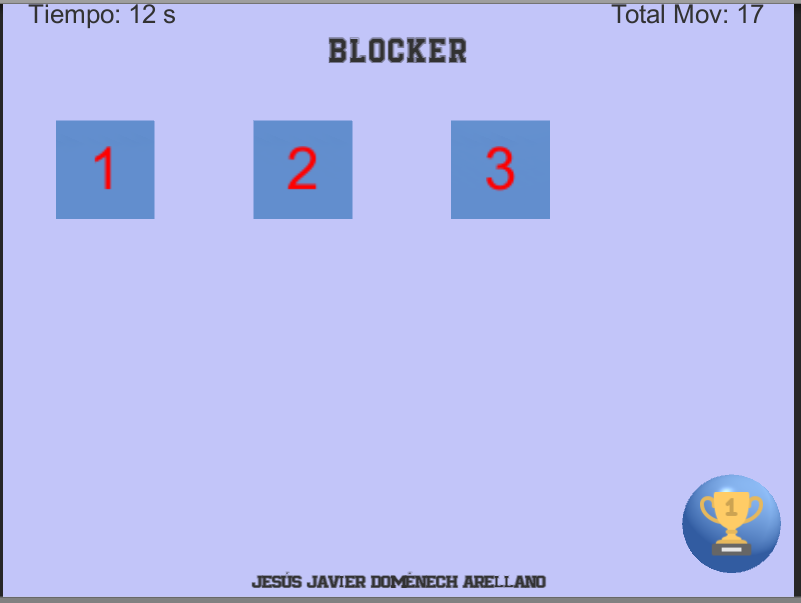
\includegraphics[scale=.4]{menu.png}
\caption{Menú de niveles (menu)}
\label{fig:menu}
\end{figure}

Inicialmente esta escena no contaba con una clase controladora, sino que cada elemento era en sí mismo su propio controlador y hacía lo que debía en función de la situación del juego. Este es el modo en el que funcionan los botones de acceso a los diferentes niveles:\\

Al cargar la escena se crean los 8 botones para los posibles niveles y estos preguntan si pueden seguir existiendo comparando el nivel al que representan y el nivel máximo desbloqueado. En caso de no estar desbloqueado es el mismo el que se autodestruye. \\

Cuando pinchamos uno de estos niveles, lo que hace es modificar una serie de variables pertenecientes al \emph{Model} de datos del juego donde indica, el XML que debe cargar, el player que debe jugar y el tiempo máximo, después de preparar estas variables manda cargar la escena de juego (denominada \emph{blocker}). \\

Al añadir a la escena los resúmenes de estadísticas, por simplicidad, añadí una clase que los gestionara, obtiene del \emph{Model} de datos del juego las puntuaciones, calcula el total y modifica los dos \emph{text}.\\

En lo referente al botón de récords, se explica en la Sección \ref{subsec:navegacion}.
\newpage
\subsection{Juego (blocker)}
Esta escena, Figura \ref{fig:juego}, es la que hace que el juego se pueda llamar juego. Se trata de una escena genérica que carga los diferentes niveles a partir de un XML y una serie de variables obtenidas del \emph{Model} de datos del juego.

\begin{figure}[h!]
\centering
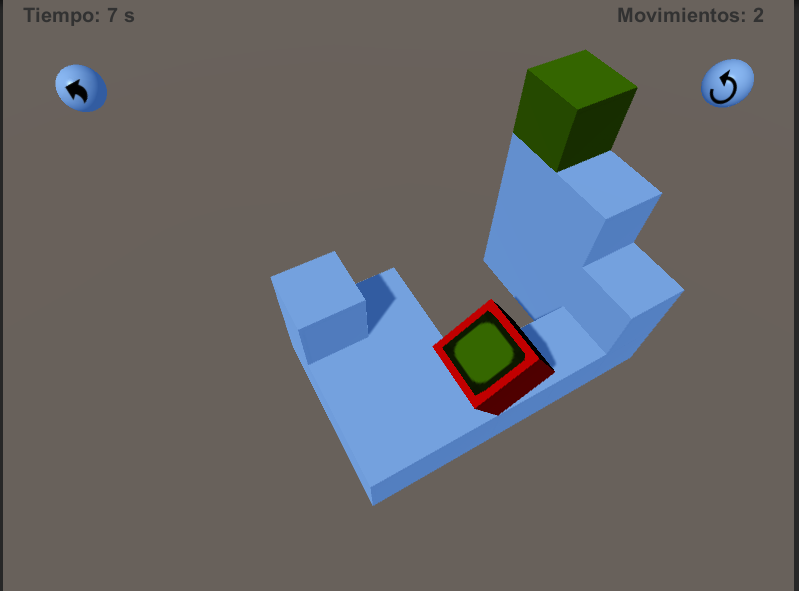
\includegraphics[scale=.4]{juego.png}
\caption{Juego}
\label{fig:juego}
\end{figure}

\subsubsection{Mapa}
La construcción del mapa está basada en la última práctica de la asignatura, de hecho hay funciones en el código con comentarios del tipo "\emph{heredada...}" que no se han tocado aunque podían haberse borrado u optimizado para el problema que se necesitaba en esta ocasión. \\

Por estar basada en la práctica de \emph{Omega Mage}, el mapa es un XML donde esta la información necesaria para pintarlo. Como se puede apreciar en la Figura \ref{fig:xml} la información es:
\begin{itemize}
    \item Identificación del nivel (\emph{num}).
    \item Posición de inicio del jugador (\emph{x\_start, y\_start}).
    \item Posición de la casilla objetivo (\emph{x\_goal, y\_goal}).
    \item Altura de cada coordenada.
\end{itemize}

La altura de salida del jugador, y la altura de la posición de la casilla objetivo dependerá de la altura que tenga el mapa en esa posición.\\

\begin{figure}[h!]
\centering
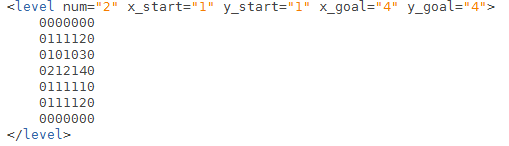
\includegraphics[scale=.9]{xml.png}
\caption{XML nivel 2}
\label{fig:xml}
\end{figure}

Data esta información la clase \emph{LayoutTiles} instancia una \emph{BaldosaPrefab} en cada coordenada indicada y si la altura es más de uno instanciará una baldosa encima de otra. Por otro lado, si estamos en la altura máxima de una coordenada se comprueba si es la casilla objetivo en cuyo caso se instanciará un \emph{GoalPrefab}, la diferencia entre ambas es simplemente el color. \\

Después de pintar el mapa, se procede a pasar la información del mismo a la clase \emph{Game} que se encargará de gestionar el mapa lógico del juego y de colocar al jugador en las coordenadas adecuadas partiendo del \emph{Prefab} almacenado en el \emph{Model} de datos del juego. 

\subsubsection{Cámara}
La cámara se presenta en proyección perspectiva para dar ese efecto de 3D. Colocar la cámara ha sido un verdadero quebradero de cabeza, dado que cada nivel tenía su posición idónea. Al final se ha ajustado a mano tras varios "pruebaYerror".\\

Se plante la posibilidad de moverla con el jugador tal y como hicimos en la práctica \emph{Mission Demolition} pero este comentario queda como mejora a añadir si en algún momento decido seguir con el juego. No lo he llevado a cabo por parecerme más interesante jugar con diferentes tipos de piezas.

\subsubsection{Puntuaciones}
\label{subsec:puntos}
Fácil, el \emph{Model} de datos del juego tiene dos arrays de 8 posiciones, una por nivel, donde se almacena el mejor tiempo y la mejor cantidad de movimientos por cada nivel. Cada vez que el jugador es movido se suma uno a una variable local del nivel que indica los movimientos del juego actual y también se va descontando el tiempo. Si el jugador consigue superar el nivel con éxito se actualizan los arrays cambiando los récord si ha mejorado los existentes.

\subsubsection{Jugador}
Lo mejor de esta escena para el final. La clase \emph{Player} es, sin lugar a dudas, a la que más tiempo he dedicado y por tanto de la que estoy más orgulloso y también la que más \emph{bugs} tiene.\footnote{A medida que voy jugando encuentro más.}\\

El jugador, como he repetido muchas veces, puede ser un cubo o tener dos pisos, he incluso esta pensado para soportar N pisos de altura, pero no todo funciona bien. Al principio iba a ser todo muy general, pero la fecha de entrega apremiaba y algunas cosas han quedado cableadas, haciendo que la figura de más de un piso no pueda subir bien escalones correctamente\footnote{Por eso, no hay niveles con la figura de dos pisos en los que tenga que subir o bajar.}.\\

Toda la clase del jugador se ha convertido casi en un controlador de la escena, suplantando parcialmente a la clase \emph{Game} que mencionaba anteriormente. Esto no es del todo malo dado que la escena solo existirá mientras exista el jugador y solo habrá un jugador por escena. \\

El jugador se ha implementado como una máquina de estados:\\
\textsc{public enum StMov \{Parado,Mov,Caer,Morir,Ganar\};}\\
Con ella podemos hacer que el jugador se mueva de manera progresiva. Tarea que no es del todo sencilla, y para nada trivial cuando hay más de un nivel de altura en la figura.\\

\textbf{¿Cómo hacer que se mueva?}
La idea si que es sencilla: tenemos que rotar sobre la arista que este en la dirección en la que queremos movernos. Para hacer esto, es necesario calcular el punto de rotación y el ángulo a girar y es aquí donde empieza a complicarse la cosa. \\

¿Qué representa decir que quieres ir adelante? Hay que dejar fijo si adelante es una posición relativa al jugador o al mapa. Y dado que he dejado la cámara en un lugar fijo he decidido que las direcciones son relativas al mapa, entonces pulsar la tecla hacia adelante puede significar poner la figura en pie o rodarla por el suelo en función de los pasos hechos anteriormente.\\

\begin{figure}[h!]
\centering
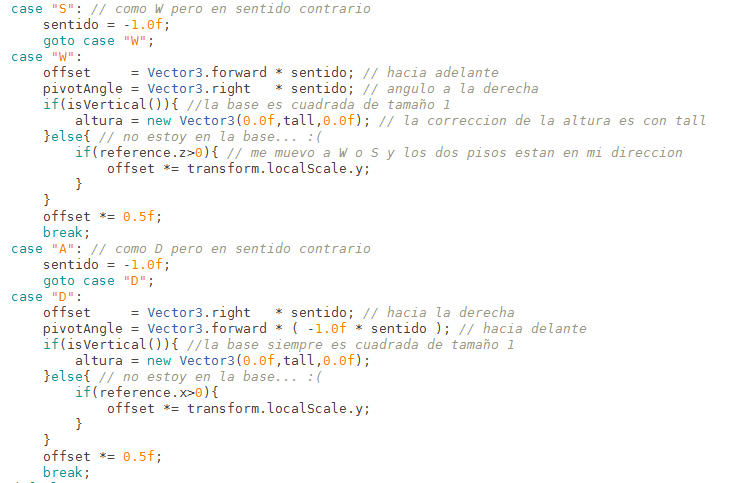
\includegraphics[scale=.75]{codigo.png}
\caption{Cálculo del Pivote}
\label{fig:codigo}
\end{figure}

Tenemos que calcular el punto de giro y la dirección es relativa al mapa, ¿Cómo lo hacemos? la idea es coger la \emph{position} del jugador y bajarla a la base y luego desplazarla hacia la arista que nos indique la dirección. Bajarla a la base dependerá de si la figura está en pie o no dado que tendremos que bajar una altura o media y moverla hacia la arista ocurre lo mismo si justo queremos movernos hacia el sentido largo de nuestra figura la cuenta se complica. Tras muchos experimentos el código final queda bastante simplificado y casi parece trivial, tal y como puede apreciarse en la figura \ref{fig:codigo}. Posteriormente se realiza la cuenta para calcular el punto de giro:

$$ pivotPoint = transform.position - altura + offset; $$

Pero esto no es todo, la casilla destino hemos supuesto que estaba a la misma altura, pero la gracia es que no siempre será así por lo que se plantean dos problemas:
\begin{itemize}
    \item \textbf{Bajar:} El punto de giro queda en el mismo lugar pero la cantidad de giro ha de ser mayor, en lugar de girar 90 grados necesitamos girar 180.
    \item \textbf{Subir:} La diferencia es que la arista sobre la que debemos girar es la superior en lugar la inferior por tanto en lugar de restar la altura a la posición del jugador se la debemos sumar y la cantidad de giro también deben ser 180 grados.
\end{itemize}
Para entender estas situaciones, lo mejor es hacer un cubo de papel y ponerse a jugar. Por supuesto, la figura sólo puede subir escalones de una altura. \\

Hasta aquí todo va bien, las figuras lo hacen sin ningún problema o casi... No hemos hablado de que pasa si la figura al subir necesita dos espacios y no los hay, se plantean tantos posibles casos y de tantas maneras que no he sido capaz de generalizarlo y tampoco el controlar que pasa si parte de mi figura queda volando o encima de un agujero. Por lo que en los niveles presentados no se da el caso. \\

Todos estos cálculos se realizan cuando el jugador esta en el estado \textsc{Parado}, y una vez están listos se pasa al estado \textsc{Mov}, en los que se realiza la rotación siguiendo el código de la Figura \ref{fig:mover}. Donde se aprecia que el movimiento se hace de manera progresiva hasta llegar al límite

\begin{figure}[h!]
\centering
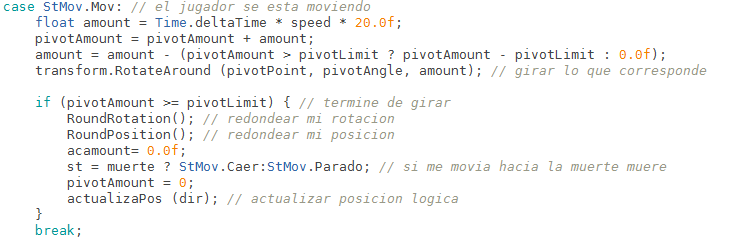
\includegraphics[scale=.75]{mover.png}
\caption{Código de movimiento}
\label{fig:mover}
\end{figure}

Después de haber hablado del movimiento queda la caída, ganar y morir. Estos dos estados son muy sencillos: en la caída se activa la gravedad y desactiva el kinematic unity hace el resto y después de caer un poco se pasa al estado morir; en ganar se actualizan los récord si corresponde y después se mata al jugador; y en morir simplemente se destruye el jugador y carga la escena del menú.



\newpage
\subsection{Récords (highscore)}
Esta es una escena muy sencilla, simplemente está compuesta por una clase que imprime los dos arrays de puntuaciones del \emph{Model} de datos del juego, explicados en la Sección \ref{subsec:puntos}, en un \emph{text}.\\

\begin{figure}[h!]
\centering
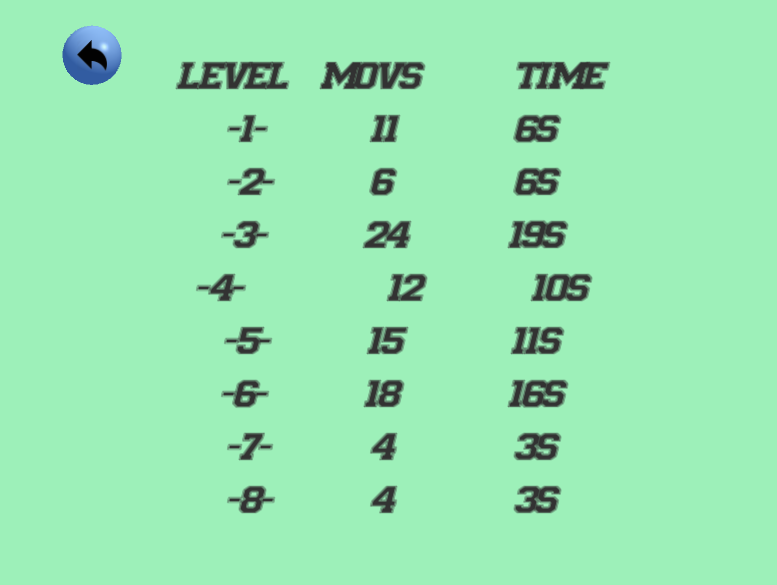
\includegraphics[scale=.4]{highscore.png}
\caption{Escena de puntuaciones (no son las mejores que he obtenido).}
\label{fig:highscore}
\end{figure}

Como dato peculiar se puede hacer notar que el tamaño de fuente de esta escena varía en función del tamaño de la pantalla, aunque la ventana está escalada a 4:3 el \emph{fontsize} no escala. Los GUI Text tienen una opción denominada "\emph{best fit}", pero no es todo lo "\emph{best}" que se podría desear, por lo que es necesario escribir unas líneas para modificar el tamaño dinamicamente.\\

Estas líneas tienen en cuenta 3 detalles:
\begin{itemize}
    \item Ancho de pantalla.
    \item Alto de pantalla.
    \item Alto del texto, sólo 9 líneas (título y 8 niveles).
\end{itemize}
Con estos tres valores se realiza la cuenta y se obtiene el tamaño idóneo para el texto, esta "cuenta" dice así:

$$ fontsize = \frac{min( ancho, \frac{alto}{9})}{Ratio} $$

El Ratio se utiliza para ajustar, la reducción del texto.\\

Por otra parte está el botón de volver al menú, explicado en la Sección \ref{subsec:navegacion}.
\newpage
\subsection{Navegación entre Escenas}
\label{subsec:navegacion}

He hablado en muchas ocasiones del \emph{Model} de datos del juego, este es una clase, Figura \ref{fig:model} que permanece accesible durante toda la vida del programa. En ella se almacena, la configuración del nivel, el nivel máximo y los récord. \\

\begin{figure}[h!]
\centering
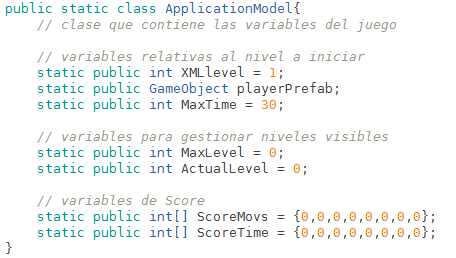
\includegraphics[scale=.75]{model.png}
\caption{Clase ApplicationModel}
\label{fig:model}
\end{figure}

En todas las escenas tenemos una serie de esferas que nos permiten tener un poco de navegación entre escenas, la forma de implementarlas es muy similar a los cubos de niveles solo que no modifican el \emph{Model}. \\

Hay tres tipos:
\begin{itemize}
    \item \textbf{Atrás:} Una flecha que nos devuelve a la escena menú.
    \item \textbf{Repetir:} Una flecha circular que vuelve a cargar el nivel actual de juego.
    \item \textbf{Récord:} Una imagen de una copa que nos lleva a la escena donde se mostrarán los récord de cada nivel.
\end{itemize}

\newpage
\section{Conclusión}
Como conclusión y aprendizaje decir que he disfrutado en el desarrollo de este videojuego aunque en algunas ocasiones ha llegado a frustrarme ver que la figura se movía como quería ella y no yo. \\

Pese a todo, en ningún momento yo diría que el juego está completo (con lo que eso implica), soy consciente de los muchos puntos posibles de mejora y tareas pendientes ha realizar, especialmente con la figura de dos pisos, pero aún así considero que ha quedado una bonita primera versión jugable, con al menos un bug\footnote{El bug se encuentra en los niveles 7 y 8.}.\\

Tal y como indico en la introducción, existe un video "gameplay"\footnote{Yo pasandome el juego.} en youtube \emph{https://youtu.be/gZ1T0LnGGtw}\\

---------------------------------------------------------------------\\


\emph{"No te avergüences de tus debilidades ya que esas son tus fortalezas."}

\end{document}
